\chapter{Numerical Methods}

This chapter discusses the Smoothed Particle Hydrodynamics (SPH) and the Discrete Element Method (DEM) numerical methods.

\section{Smoothed Particle Hydrodynamics}

The Smoothed Particle Hydrodynamics (SPH) numerical method was developed in the late 1970s \cite{gingold_monaghan} for tackling problems in Astrophysics which involved arbitrarily moving, three dimensional fluid masses in the absence of boundaries; the equations represented below are discussed in this framework. Since it's inception however, the SPH method has come a long way and has been used in numerous fields such as magneto-hydrodynamics, multi-phase flows, quasi-incompressible flows, gravity currents, flow through porous media, heat conduction, shock simulations, heat transfer and mass flow, explosion phenomenon, high/hyper velocity impact problems etc. \cite{liu_liu}.

\begin{figure}[htb!]
\centering
\setlength\fboxsep{0pt}
      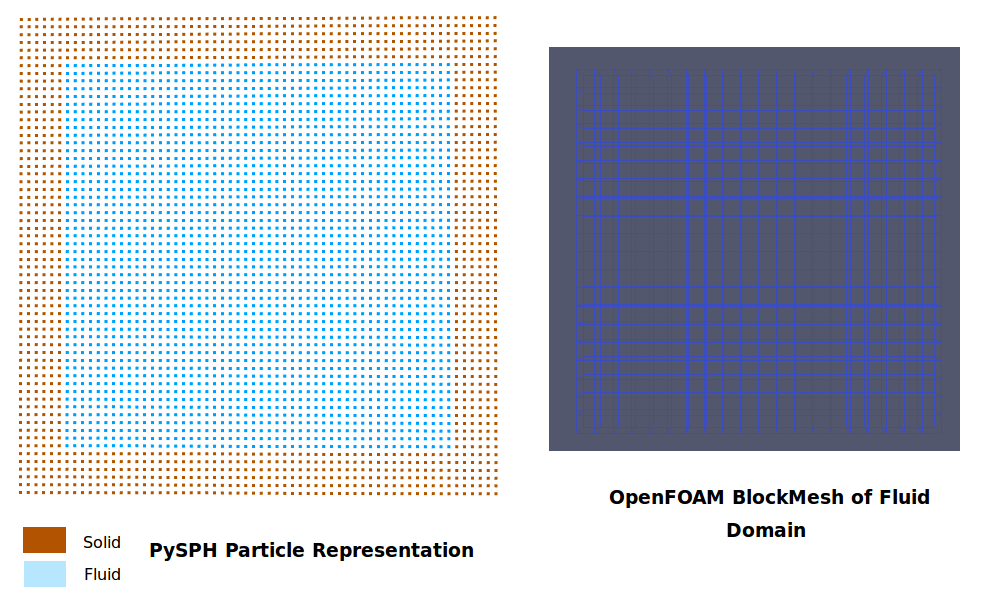
\includegraphics[width=5in, height=2.5in]{figures/particle_rep.png}
\caption{{\small{Domain Discretization in the SPH and FVM numerical Methods}}}
\label{fig:particle_representation}
\end{figure}

The SPH method takes into account the motion of a set of points whose velocity and thermal energy is known at all times. These points are also assigned a mass, and hence, are called as ``Particles''\cite{monaghan_intro}. Thus Domain discretization is achieved by means of a ``Particle Representation'' which describes the fluid domain. Such a representation allows for a completely arbitrary initial distribution of particles, with no explicit requirement of inter-particle connectivity, thereby qualifying SPH to be a Mesh-Free numerical method. Figure ~\ref{fig:particle_representation} shows the domain discretization for a simple incompressible flow problem (the lid-driven cavity) for solving equations with the SPH method and the Finite Volume Method (FVM). The software tools used for generating the representations are PySPH \cite{prabhu_puri} and OpenFOAM \cite{foam} respectively.

Every particle has all the field variables of a Continuum Point Particle associated with it\footnote{``Particles'' are an outcome of the application of SPH on the matter continuum;``Point Particles'' are the basic building blocks of the Continuum approximation.}. The SPH method represents the governing differential equations as a set of difference equations with the dependant and independent variables of the differential equations being related to those ~ of ~ the ~ difference ~ equation ~ by ~ means ~ of ~ a ~``Particle ~ Approximation'' ~ \cite{sph:volieu}\\\cite{liu_liu} detailed below.

\subsection{Particle Approximation}\label{kappa}

Consider an arbitrary scalar field A(\textbf{r},\textit{t}) associated with a particle having position vector \textbf{r} at time \textit{t}. This field can be written as a spatial convolution with the Dirac Distribution $\delta$ as, 

\begin{eqnarray} \label{eq:dirac}
 A(\textbf{r},\textit{t}) &=& (A\ast \delta)(\textbf{r},t) \nonumber \\
                          &=& \int_{\varOmega} A(\textbf{r'},t) \delta (\textbf{r - r'}) d^{3}\textbf{r'} 
\end{eqnarray}

where $\varOmega$ represents the domain of the Continuum. 

Practically, the Dirac Distribution is approached by use of Interpolation Kernels\footnote{The terms Interpolation Kernels, Mollifiers, Smoothing Kernels etc. are used interchangeably in literature.}, denoted as \textit{w$_h$}(\textbf{r - r'}). These kernels could have a compact or an infinite support and have associated with them a Smoothing Parameter ``h'' which controls the sphere of influence of each particle. For a kernel with a compact support, if the point particle under consideration were imagined to be at the center of an n-dimensional hypersphere (n$=$3 in this particular case) of radius, \textit{r}$=\kappa$h ($\kappa$ being a multiplying constant), then all those point particles which lie within this hypersphere would contribute to the properties of the point particle at the center; for a kernel with an infinite support, the effect of point particles at larger distances from the center of the hypersphere would diminish. Thus, the continuous domain of integration $\varOmega$ is reduced to that of the the hypersphere, $\varOmega_r$. (Properties of Kernels are discussed in \ref{ssec:kernels}). 

\begin{figure}[htb!]
\centering
\setlength\fboxsep{0pt}
      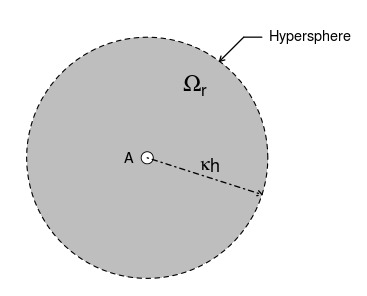
\includegraphics[scale=0.6]{figures/SpInfContinuous_R.png}
\caption{{\small{Sphere of Influence of a Point Particle A centred at the Origin of a 2D Hypersphere}}}
\label{fig:sphere_influence}
\end{figure}
\newpage
Equation \eqref{eq:dirac} can be rewritten, by making the ``Kernel Approximation'',  as,

\begin{eqnarray} \label{eq:continuous-approximation}
 A(\textbf{r},t) \approx [A]_{c}(\textbf{r},t)= \int_{\varOmega_r} A(\textbf{r'},t) \textit{w$_h$(\textbf{r - r'})} d^{3}\textbf{r'}
\end{eqnarray}

Equation \eqref{eq:continuous-approximation} is called the Kernel/Continuous Approximation of the field A(\textbf{r},\textit{t}) which is introduced due to the use of the Kernel function \textit{w$_h$}(\textbf{r - r'}).

Thereafter, a discrete interpolation is obtained by expressing Equation \ref{eq:continuous-approximation} as a Riemann sum over all the particles falling within the hypersphere, i.e.

\begin{eqnarray} \label{eq:particle-approximation}
     [A]_{c}(\textbf{r},t) &=& \int_{\varOmega_r} A(\textbf{r'},t) \textit{w$_h$(\textbf{r - r'})} d^{3}\textbf{r'} \nonumber \\
     &\approx & \sum_{b}A(\textbf{$\bf{r}_b$},t)~\textit{w$_h$}(\textbf{$|\bf{r}-\bf{r}_b |$}) ~ \textit{V$_b$} = [A]_{d} \nonumber \\
     \therefore [A]_{d} &=& \left( \sum_{b}A(\textbf{$\bf{r}_b$},t)~\textit{w$_h$}(\textbf{$|\bf{r}_{ab} |$}) ~ \textit{V$_b$}\right) ,
     \forall a \in  \varOmega_r , \textbf{r}_{ab} = \textbf{r}_{a} - \textbf{r}_{b}
\end{eqnarray}

The job of keeping track of all the particles ``b'' which influence any particle ``a'' is designated to the a Nearest Neighbour Particle Search (NNPS) Algorithm. Although the NNPS is the main work-horse of any SPH simulation, its description and implementations is beyond the scope of this work. 

To conclude, it should be noted that although the treatment given above is for an arbitrary scalar field, the same can be extended to an arbitrary vector field as well, by treating each component individually. Furthermore, the above treatment is valid only for the bulk of the fluid in the absence of any boundaries; treatment of boundaries within SPH is addressed separately and is not discussed in this work.

\subsection{Kernel Functions} \label{ssec:kernels}

This section describes the main properties a kernel function should possess in order to be able to produce the first order accurate description given in Equation \eqref{eq:continuous-approximation}.

\subsubsection{Kernel Properties}
 The two conditions on imposed a kernel function are:
 \begin{eqnarray} \label{eq:kernel-props1} 
  \int_{\varOmega_0} \textit{w$_h(\widetilde{r}) ~d^{3}\widetilde{r}$} = 1
 \end{eqnarray}
 and
 \begin{eqnarray}\label{eq:kernel-props2}
  \int_{\varOmega_0} \textit{w$_h(\widetilde{r})~ \widetilde{r}~ d^{3}\widetilde{r}$} = 0 
 \end{eqnarray} 
 where ${\varOmega_0}$ is ${\varOmega_r}$ translated to the origin \textbf{0}.
 

 Equation \eqref{eq:kernel-props1} stipulates that the zeroth order moment of the Kernel be 1, like that of the Dirac $\delta$; \eqref{eq:kernel-props2} stipulates that the first order moment (i.e. the Mean or the Expectation) be zero. 
 
 There are various ways in which, mathematically, one could construct functions which satisfy the above two requirements. However, in general, the simplest way to satisfy \eqref{eq:kernel-props2} is by using a Symmetric function (which could be normalized to ensure \eqref{eq:kernel-props1} is satified as well). \newpage This gives us the following relation for the Kernel function:
 
 \begin{eqnarray}\label{eq:kernel-symmetry}
  \textit{w$_h(\widetilde{r}$)} = \textit{w$_h(-\widetilde{r}$)}
 \end{eqnarray}

\subsubsection{Action of Differential Operators}

 Consider the application of the Kernel Approximation of Equation \eqref{eq:continuous-approximation} of the gradient of a scalar field as given below \cite{sph:volieu}: 
 
 \begin{eqnarray} \label{eq:diff_operator}
 \left[\textbf{grad}~A\right]_{c}(\textbf{r},t) &=& \int_{\varOmega_r} \frac{\partial A(\textbf{r'},t)}{\partial \textbf{r'}} \textit{w$_h$(\textbf{r - r'})} d^{3}\textbf{r'} \nonumber\\
 &=& \int_{\varOmega_r} \frac{\partial}{\partial \textbf{r'}}\left[A(\textbf{r'},t) \textit{w$_h$(\textbf{r - r'})} \right]d^{3}\textbf{r'} \\
 &-& \int_{\varOmega_r} A(\textbf{r'},t) \frac{\partial w_h(\textbf{r - r'}) }{\partial \textbf{r'}} d^{3}\textbf{r'} \nonumber
 \end{eqnarray}
 
 The first term of Equation \eqref{eq:diff_operator} can be expressed in terms of a surface integral by applying Guass' Divergence Theorem which vanishes in the bulk of the fluid in the absence of any boundaries \cite{sph:volieu}. 
 
 The second term can be expressed as $$\int_{\varOmega_r} A(\textbf{r'},t) \frac{\partial w_h(\textbf{r - r'}) }{\partial \textbf{r}} d^{3}\textbf{r'}$$ by making use of the identity $$\frac{\partial w_h(\textbf{r - r'}) }{\partial \textbf{r'}} = -\frac{\partial w_h(\textbf{r - r'}) }{\partial \textbf{r}}$$
 
 Hence, we have 
 \begin{eqnarray}\label{eq:grad}
 \left[\textbf{grad}~A\right]_{c}(\textbf{r},t) = \int_{\varOmega_r} A(\textbf{r'},t) \frac{\partial w_h(\textbf{r - r'}) }{\partial \textbf{r}} d^{3}\textbf{r'} = \int_{\varOmega_r} A(\textbf{r'},t) ~\nabla\left[w_h(\textbf{r - r'})\right] d^{3}\textbf{r'} 
 \end{eqnarray}  
 
 Analogously, the following relation can be obtained, 
 \begin{eqnarray}\label{eq:div}
 \left[\textbf{div}~A\right]_{c}(\textbf{r},t) =  \int_{\varOmega_r} A(\textbf{r'},t) \cdot ~\nabla \left[w_h(\textbf{r - r'})\right] d^{3}\textbf{r'} 
 \end{eqnarray}
 
 Finally, by applying the Particle approximation, we can express the Equations \eqref{eq:grad} and \eqref{eq:div} as Riemann Sums much like those given by Equation \eqref{eq:particle-approximation} to obtain algebraic expressions for solving simultaneously.

\section{Discrete Element Method} \label{sec:DEM}

The Discrete Element Method \cite{mishra} is a numerical method that allows finite rotations and displacements of discrete bodies which interact with their nearest neighbours by means of local Contact Laws where the loss of contact and the formation of new contacts occur as the simulation progresses. To track the position of the solid rigid bodies, the interacting bodies (also called as particles) are modelled as a dynamic process in which contacts are broken and formed. In order to estimate the reaction force due to interaction or collision between particles ``Hard'' or ``Soft'' Contact models are employed. Hard Contact models rely on the phenomenon of Restitution and require information of the Coefficient of Restitution between the interacting particles to be supplied as a model parameter. Since obtaining information about the Coefficient of Restitution experimentally is quite an arduous task, Hard Contact models are not widely used. Soft Contact Models, on the other hand, allow the particles to overlap during contact. The amount and rate of overlap gives rise to an incremental force which is tracked in each calculation cycle. Thereafter, numerical integration of Newton's Second Law of Motion gives the linear and angular velocities of the system; a second integration gives the linear and angular displacements.

The DEM method requires the net unbalanced forces to be calculated for all particles on account of interaction with all other particles within the system. In the case of an interaction, the resulting force will be non-zero, otherwise the resulting force will be zero for that particular pair of interacting particles. However, for a system comprising of \textbf{N} particles, this would result into keeping track of $\dfrac{{\bf{N}} \times {\bf{(N-1)}}}{2}$ interactions. In order to improve the efficiency of the computation, the entire working area is divided into squares (or cubes depending on whether a 2/3 dimensional implementation is being considered). Such a procedure is called as ``Boxing'' in the DEM literature. Generally, the dimension of the box is the diameter\footnote{In general, DEM particles are taken to be spherical; however, there are many studies made for particles of different shapes.} of the largest particle in the system. A particle is regarded as a member in all those boxes where the corners of its circumscribing square have an entry.  A list of all the particles in a box (i.e. a Box List) is generated and only those elements which have entries in a box are considered for potential contact. Thereafter, soft contact models are (generally) employed, and the incremental force is computed.